\documentclass[a4paper,10pt]{article}
%-----------------------------------------------------------
\usepackage[top=0.75in, bottom=0.75in, left=0.55in, right=0.85in]{geometry}
\usepackage{graphicx}
\usepackage{url}
\usepackage{palatino}
\usepackage{tabularx}
\fontfamily{SansSerif}
\selectfont

\usepackage[T1]{fontenc}
\usepackage
%[ansinew]
[utf8]
{inputenc}

\usepackage{color}
\definecolor{mygrey}{gray}{0.75}
\textheight=9.75in
\raggedbottom

\setlength{\tabcolsep}{0in}
\newcommand{\isep}{-2 pt}
\newcommand{\lsep}{-0.5cm}
\newcommand{\psep}{-0.6cm}
\renewcommand{\labelitemii}{$\circ$}

\pagestyle{empty}
%-----------------------------------------------------------
%Custom commands
\newcommand{\resitem}[1]{\item #1 \vspace{-2pt}}
\newcommand{\resheading}[1]{{\small \colorbox{mygrey}{\begin{minipage}{0.975\textwidth}{\textbf{#1 \vphantom{p\^{E}}}}\end{minipage}}}}
\newcommand{\ressubheading}[3]{
\begin{tabular*}{6.62in}{l @{\extracolsep{\fill}} r}
	\textsc{{\textbf{#1}}} & \textsc{\textit{[#2]}} \\
\end{tabular*}\vspace{-8pt}}
%-----------------------------------------------------------


\begin{document}
\hspace{0.5cm}\\[-0.2cm]
\centering
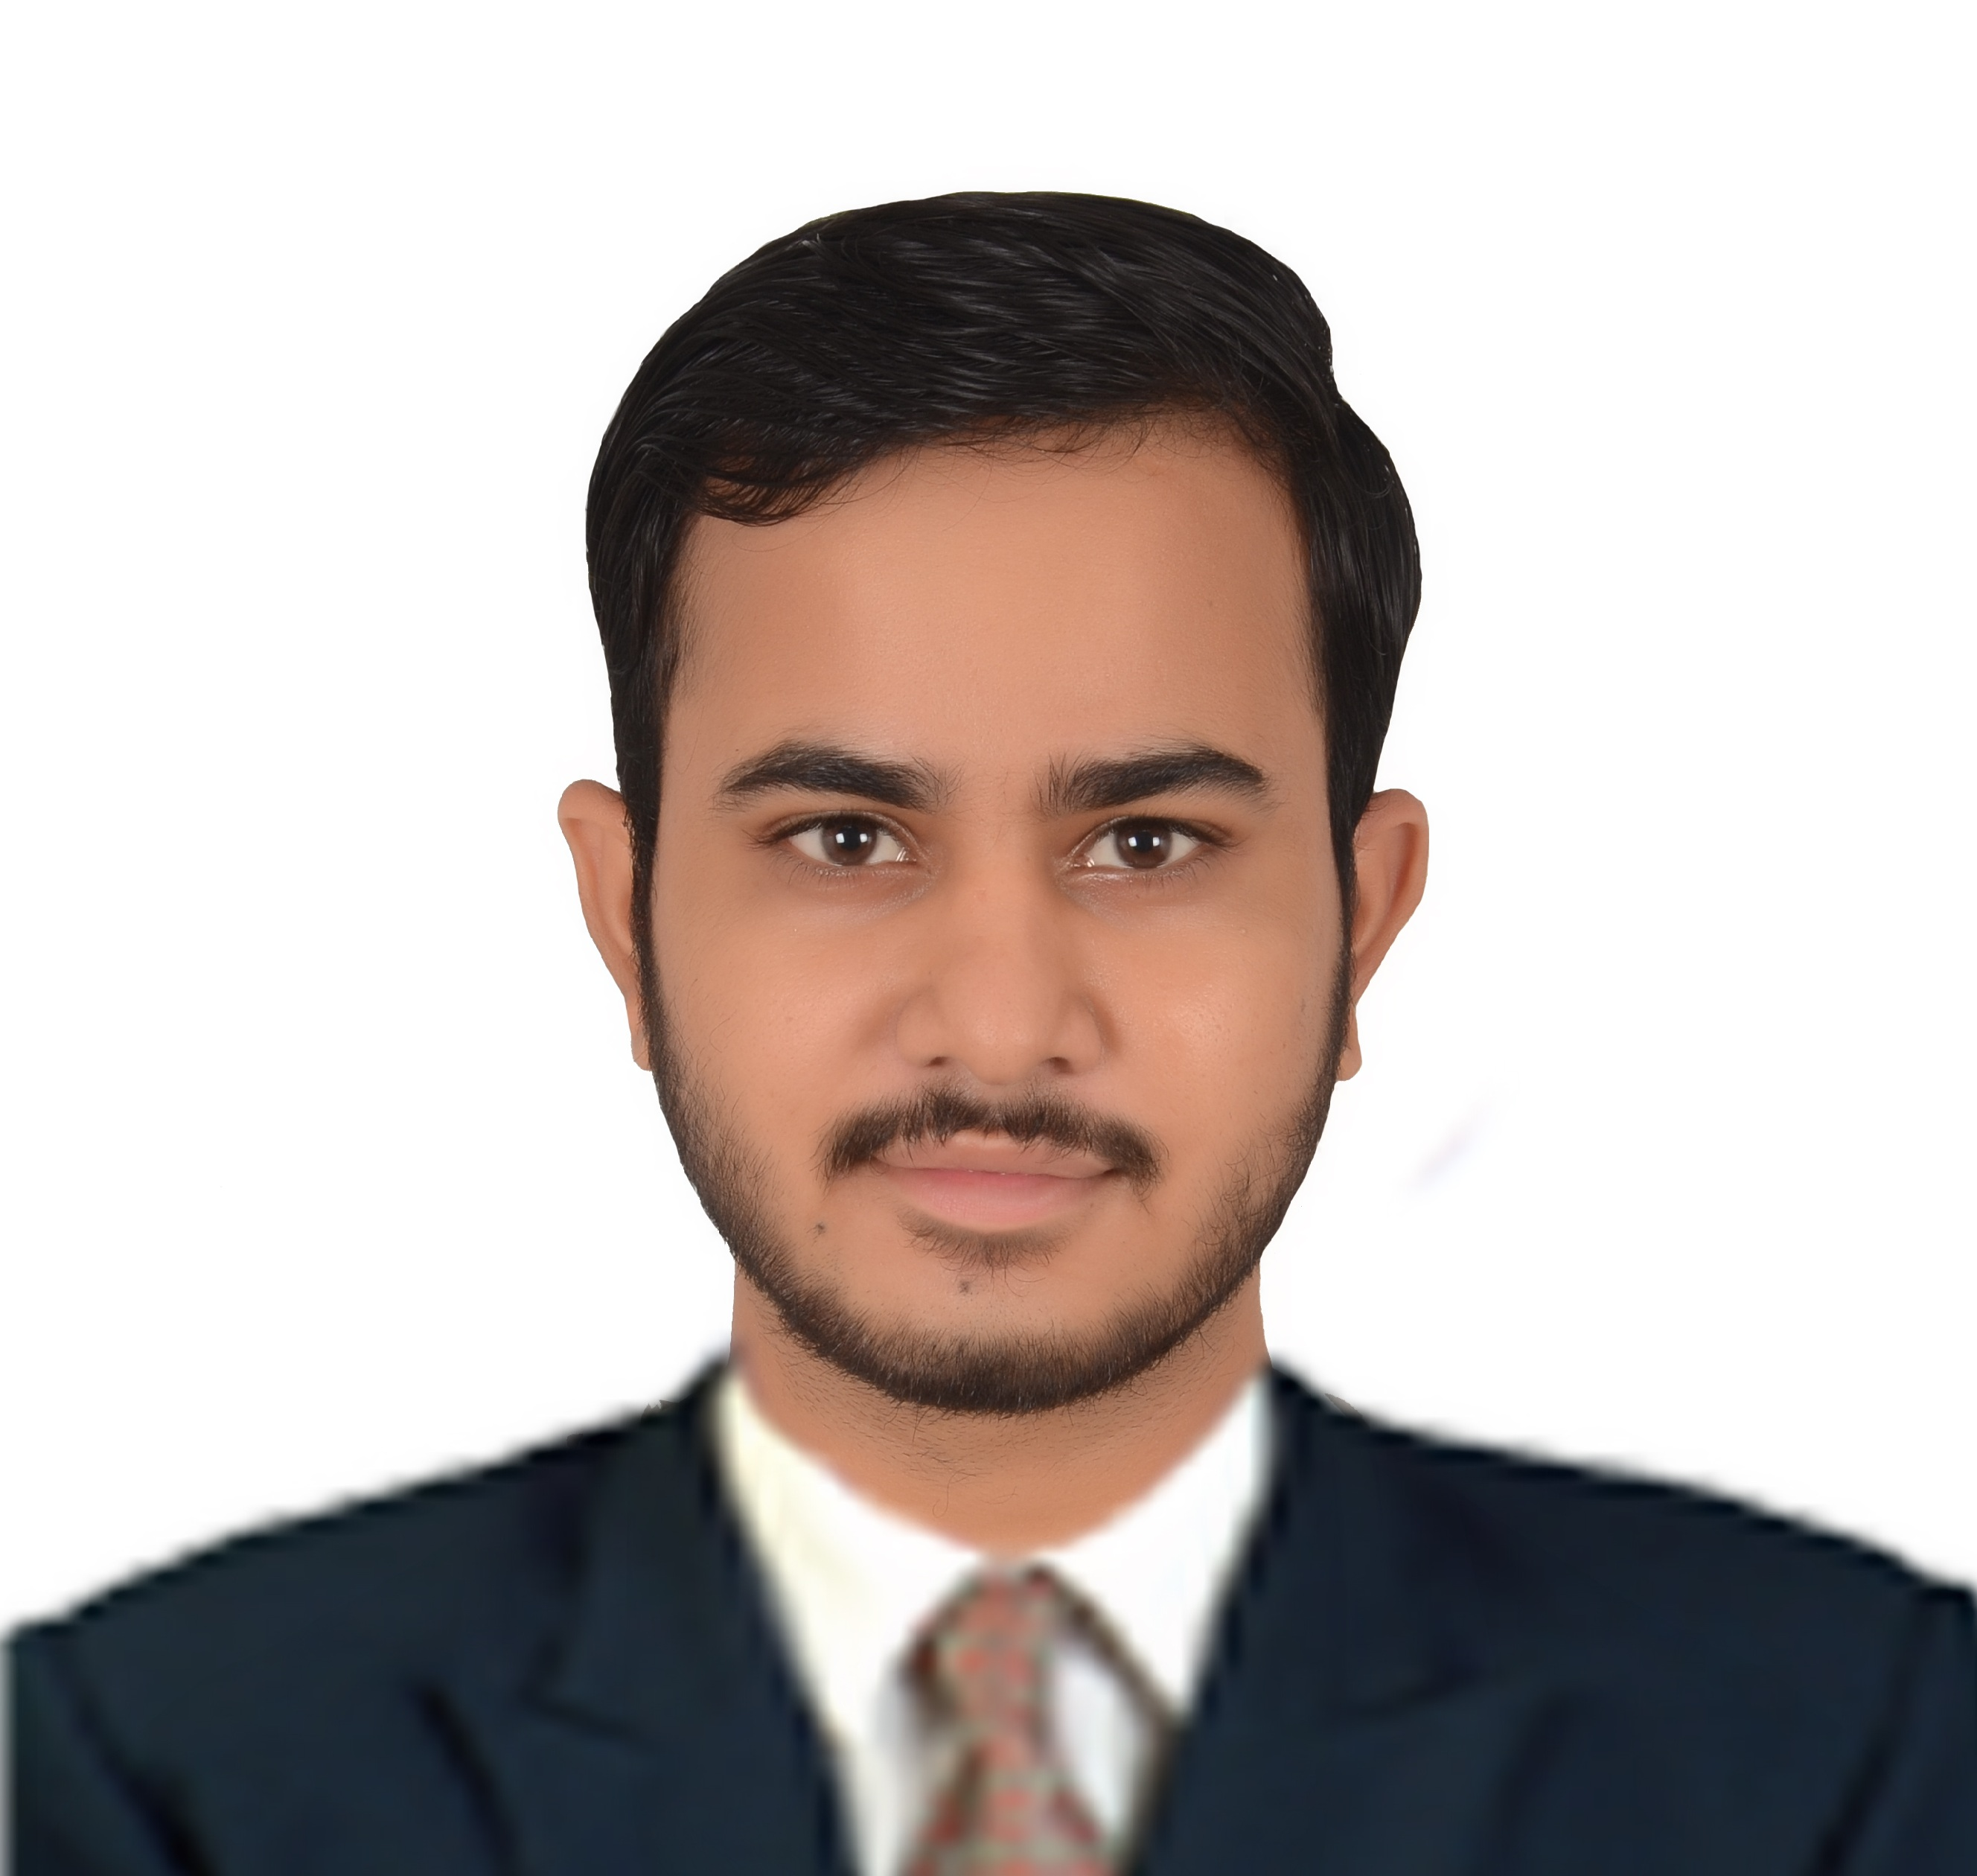
\includegraphics[scale=.2]{photo.jpg}\\
\textbf{DEVANG JOSHI} \\   
%\textbf{ADDRESS:}\\
\indent A-15 Darshanam Homes, Opp. Yash Complex, \\
\indent Nr.Narayan Gardens, New Alkapuri Road,\\
\indent Vadodara (Gujarat, INDIA) - 390021\\
\indent \textbf{Email-id :} \textbf{devang0709@gmail.com} \\
\indent \textbf{Mobile No.:} \textbf{9099002368} \\

\hspace{.2cm}\\
    \resheading {\textbf{\Large{{CAREER OBJECTIVE}}}}\\[\lsep]
\begin{itemize}
\item \noindent To utilize my technical skills for achieving the target and developing the best performance in the organization.
\end{itemize}

\resheading{\textbf{\Large{ACADEMIC DETAILS}} }\\
%\hspace{.1cm}
\begin{itemize}
\item \noindent Pursuing Bachelor of Engineering (BE) in 8th semester in Mechanical Engineering.
\end{itemize}

%\begin{table}[ht!]
%\begin{center}
\indent \begin{tabular}
{ l @{\hskip 0.15in} l @{\hskip 0.15in} l @{\hskip 0.15in} l @{\hskip 0.15in} l @{\hskip 0.15in} l }
\hline
\centering
\textbf {\centering{Sr. No.}} & \textbf{Examination} & \textbf{University/Board} & \textbf{Institute} & \textbf{Year} & \textbf{CGPA} \\
\hline
1. & SSC & CBSE & Lions English School & 2012 & 7.9 \\
2. & Diploma & GTU & Parul Institute of Engineering \&  & 2015 & 7.1\\
& & & Technology\\
3. &BE Cont. & GTU & Vadodara Institute of Engineering & 2018 & 6.61\\
\hline
\end{tabular}
%\end{center}
%\end{table}

\hspace{5cm}
\resheading{\textbf{\Large{PROJECTS}} }\\[\lsep]

\begin{itemize}
\item \underline{\Large{\textbf{Diploma Project}\\}}
\end{itemize}
\begin{itemize}
 	\begin{itemize}
 	\item \underline{\textbf{Combine Drilling \& Grinding Machine}}
 	\begin{itemize}\itemsep \isep
 	    \item \textbf{Duration} : 5th \& 6th semester
	    \item \textbf{Description} : This machine was designed of performing two different operations drilling \& grinding consequently as there working principle are same.It increses the production rate and also reduces the cost of purchasing two different machine which ultimately increases the productivity of industry. 
	    \end{itemize}
	\end{itemize}
    \end{itemize}	
    
\begin{itemize}
\item \underline{\Large{\textbf{BE Projects}}}\\
\end{itemize}
    \begin{itemize}
    \begin{itemize}
    \item \underline{\textbf{Rebar Tying Machine.}} \\
	\begin{itemize}\itemsep \isep
	\item \textbf{Duration} : 5th \& 6th semester
	\item \textbf{Description} : This machine is used to tie the reinforced bar together with the help of steel wires automatically. It helps in reducing the time of rebar tying and also helps in increasing the accuracy of the tye. With the help of his machine we can also reduce the injuries caused by the sharp steel wires while tying the rebars.
	\end{itemize}	
	
\item \underline{\textbf{Automatic Stirrup Making Machine.}}\\
	\begin{itemize}\itemsep \isep
	\item \textbf{Duration} : 7th \& 8th Semester
	\item \textbf{Description} : This machine is used to make the stirrups by bending rods to required shape and size as per the size of the beams and columns. The main objective of this project is to eliminate the manual operation of stirrup making and converting it to automation. We programmed the machine to acquire the stirrups as per the Indian Standard.
	\end{itemize}
	\end{itemize}
\end{itemize}


\resheading{\textbf{\Large{TRAINING \& INTERNSHIP}}}\\[\lsep]
\begin{itemize}
\item \noindent One day visit in the railways service station at Dahod where servicing of all type coaches and engines is been done.
\end{itemize}
\begin{itemize}
\item \noindent Issued a two months training on a designing software SOLIDWORKS from the authorized training center.
\end{itemize}
\begin{itemize}
    \item \noindent Four day certified training on PLC, HMI and Servo motor of Mitshubishi company at Ahemdabad in Mitshubishi training centre.
\end{itemize}

\resheading{\textbf{\Large{FIELDS OF INTEREST}}}\\[\lsep]
\begin{itemize}
\item \noindent Mechanical Designing
\item \noindent Manufacturing
\item \noindent Sports like Football, Cricket and Badminton.
\end{itemize}

\resheading{\textbf{\Large{TECHNICAL SKILLS}}}\\[\lsep]
\begin{itemize}
\item \noindent {Designing Software} (Autodesk Inventor and Solidworks)
\item \noindent {Worked on Various CNC Machines (like Turret center, Vertical Milling, etc.)}
\item \noindent Programmed and manufactured parts on Zmorph 3-d Printer.
\item \noindent {CNC programming via. Autodesk Inventor HSM}.
\end{itemize}

\resheading{\textbf{\Large{SOFT SKILLS}}}\\[\lsep]
\begin{itemize}
\item \noindent Problem solving ability
\item \noindent Leadership Quality
\item \noindent Team work ability
\item \noindent Finance as well as time management skill
\end{itemize}

\resheading{\textbf{\Large{EXTRA OR CO-CURRICULAR ACTIVITIES}} }\\[\lsep]
\begin{itemize}
\item \noindent I was the member of college Robocon Team of Vadodara Institute of Engineering which had {\textbf{won the National ABU Robocon-2016} }.
\item \noindent I was the member of college Robocon team which \textbf{ represented India at the Asian level in ABU Robocon contest in 2016 at Bangkok, Thailand} where we secured the position among the top 8 teams and also achieved the \textbf{"Best Design Award".}
\item \noindent  I was the member of college Robocon team of Vadodara Institute of Engineering, \textbf{participated in the ABU Robocon 2017 with two teams} at the national level and both the teams \textbf{qulified for the semifinals} and also awarded with \textbf{"Best Operator Award".}
\item \noindent Member of the college Robocon team participated in the ABU Robocon 2018 with two teams.
\item \noindent Participated and won the robotics competition named {\textbf{World Robotics Competition (WRO) 2017}} at national level.
\item \noindent Our final year project was \textbf{selected for presentation among the 35 teams from all over India} in an automation based event named {\textbf{"Mitsubishi Electric Cup 2018"}} held at Nirma University \textbf{organised by Mitsubishi Electric Pvt. Ltd.}.
\item \noindent We achieved the \textbf{Appreciation award} for our project in the \textbf{Mitsubishi Electric Cup 2018.}
\item \noindent Participated in an \textbf{e-YIC (e-Yantra Ideas Competition) 2018 held at IIT Powai} and achieved \textbf{Best Demonstration and Presentatin award \& Judges Choice award.}
\item \noindent I got \textbf{first price in an designing competition} held at R. K. University \textbf{organized by ISTE (Indian Society for Technical Education)}.
\item \noindent Also had participation certies in various technical events held in different collages during there techfests.
\item \noindent Got training on an \textbf{musical instrument TABLA for 5yrs} and also appeared for various examinations for the same.
\end{itemize}

\resheading{\textbf{\Large{PERSONAL DETAILS}}}\\[\lsep]
\begin{itemize}
\item {\textbf{Father's Name}} : Rajnikant J Joshi
\item {\textbf{Mother's Name}} : Sushma R Joshi
\item {\textbf{Sex}} : Male
\item {\textbf{Date of Birth}} : 27-September-1996
\item {\textbf{Nationality}} : Indian
\item {\textbf{Merital Status}} : Unmarried
\end{itemize}

\resheading{\textbf{\Large{REFERENCE}}}\\[\lsep]
\begin{enumerate}
    \item \noindent Dr. Jayeshkumar S. Patel\\
     Principal\\
     Vadodara Institute of Engineering\\
     Vadodara\\
     Contact number : 02653915900\\
     Email : vierorgin@yahoo.com\\
     
     \item \noindent Prof. Vimal B Patel\\
     GTU Coordinator\\
     Vadoara Institute of Engineering\\
     Vadodara\\
     Contact number : +919624560842\\
     Email : vml310@gmail.com
     
    \item \noindent Prof. Satish Bhati\\
    Assistant Professor\\
    Vadodara Institute of Engineering\\
    Vadodara\\
    Mobile : +919909959321\\
    Email : bhatisatish4045@gmail.com
\end{enumerate}

\resheading{\textbf{\Large{DECLARATION}}}\\[\lsep]
\begin{itemize}
\item \noindent “I hereby declare that all the information mentioned above is true to the best of my knowledge and belief.”
\end{itemize}

\hspace{3cm}
\begin{itemize}
    \raggedright{}
\end{itemize}
\raggedleft{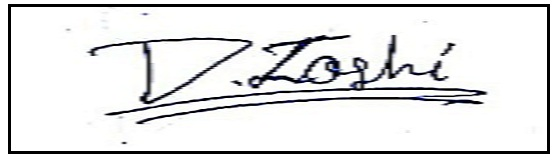
\includegraphics[scale=.2]{devang.jpg}}\\
\hspace{.2cm}
\raggedright{Date : 19/April/2018}\\\raggedleft{Your's Faithfully,}\\
\raggedleft{Devang Joshi}
\end{document}